\section{Goal of the project}
\label{sec:goal}

The \texttt{gdpr\_anonymizer} repository provides a local toolchain for video privacy preservation through instance segmentation and mask-based blurring. The workflow is intended for researchers and developers who require repeatable control over frame sampling, polygon annotation, model training, validation, and anonymization before footage is shared. Datasets and model weights remain on the host machine, and each stage is invoked through explicit command-line paths rather than embedded configuration.

The toolchain addresses a practical need in audiovisual research: sensitive regions such as persons or vehicles must be obscured without discarding the surrounding scene context. This is achieved by training a YOLO26 segmentation model on hand-labelled masks, evaluating mask quality with standard metrics, and applying Gaussian or pixelated blur inside predicted mask unions on each video frame. The software does not by itself establish legal compliance with the General Data Protection Regulation (GDPR); lawful processing and consent remain the responsibility of the data controller in the relevant jurisdiction.

\begin{figure}[htbp]
  \centering
  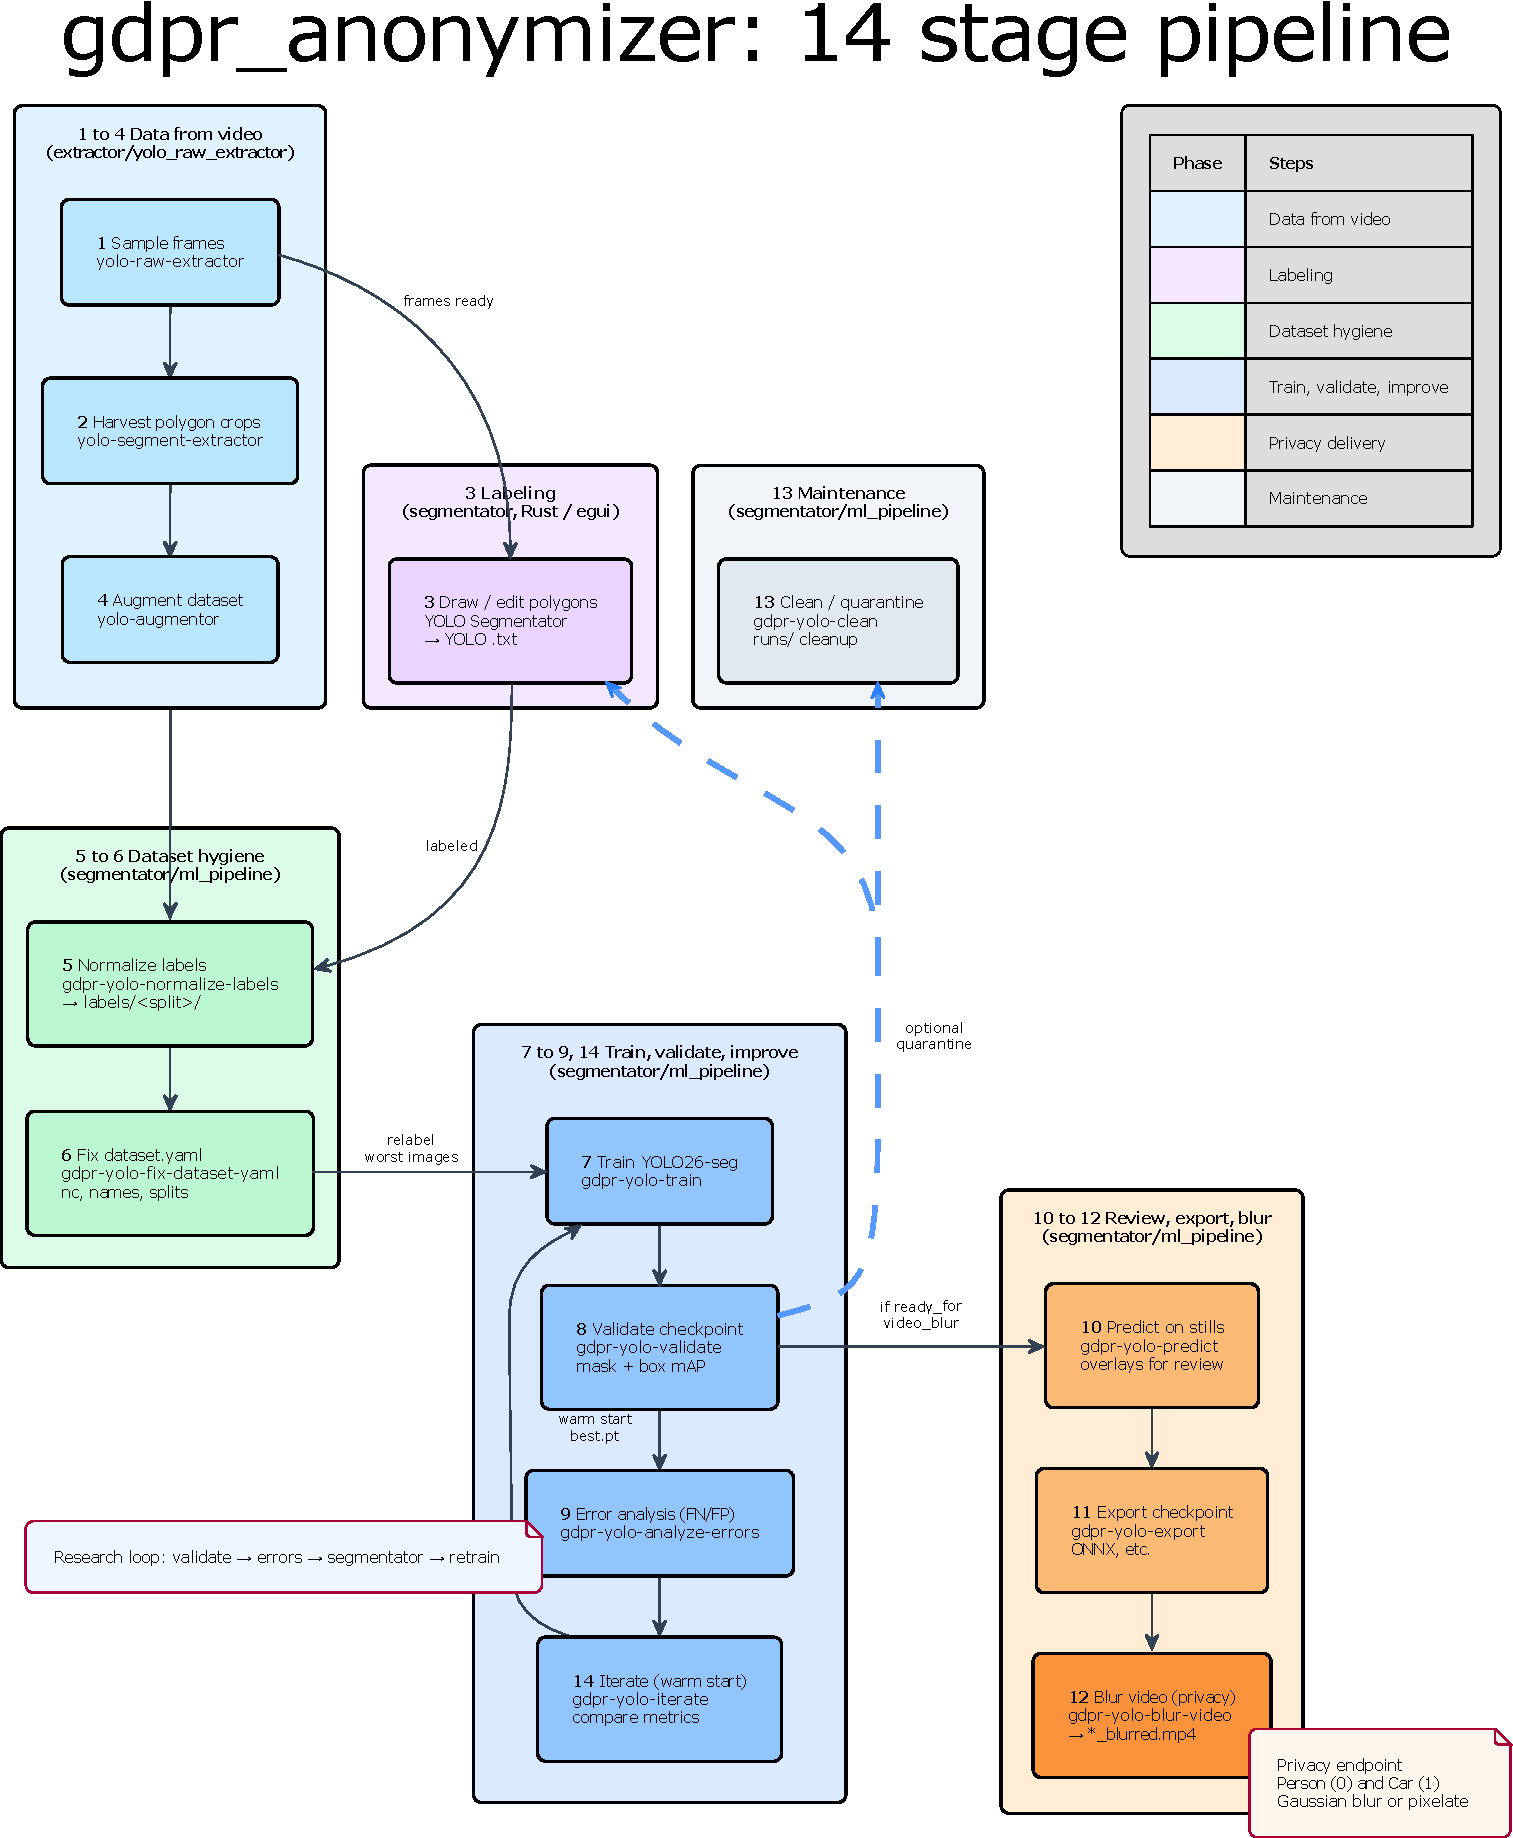
\includegraphics[width=0.88\textwidth]{images/pipeline14steps.pdf}
  \caption{Fourteen-stage privacy pipeline for the \texttt{gdpr\_anonymizer} project. Stages~1--4 correspond to the Python extractor package; stage~3 uses the Rust segmentator; stages~5--14 are provided by \texttt{segmentator/ml\_pipeline}.}
  \label{fig:pipeline14steps}
\end{figure}

Figure~\ref{fig:pipeline14steps} summarises the fourteen ordered stages from raw video to anonymised output. Steps~1--4 prepare data: frames are extracted, polygons are drawn in the desktop segmentator, segment crops are harvested for augmentation after labelling, and an augmented dataset copy is built. Steps~5--6 audit label layout and \texttt{dataset.yaml}. Steps~7--11 cover training, validation, error analysis, still-image prediction, and checkpoint export. Steps~12--14 deliver video blur, dataset or run-folder cleaning, and warm-started training iteration with metric comparison.

\begin{figure}[htbp]
  \centering
  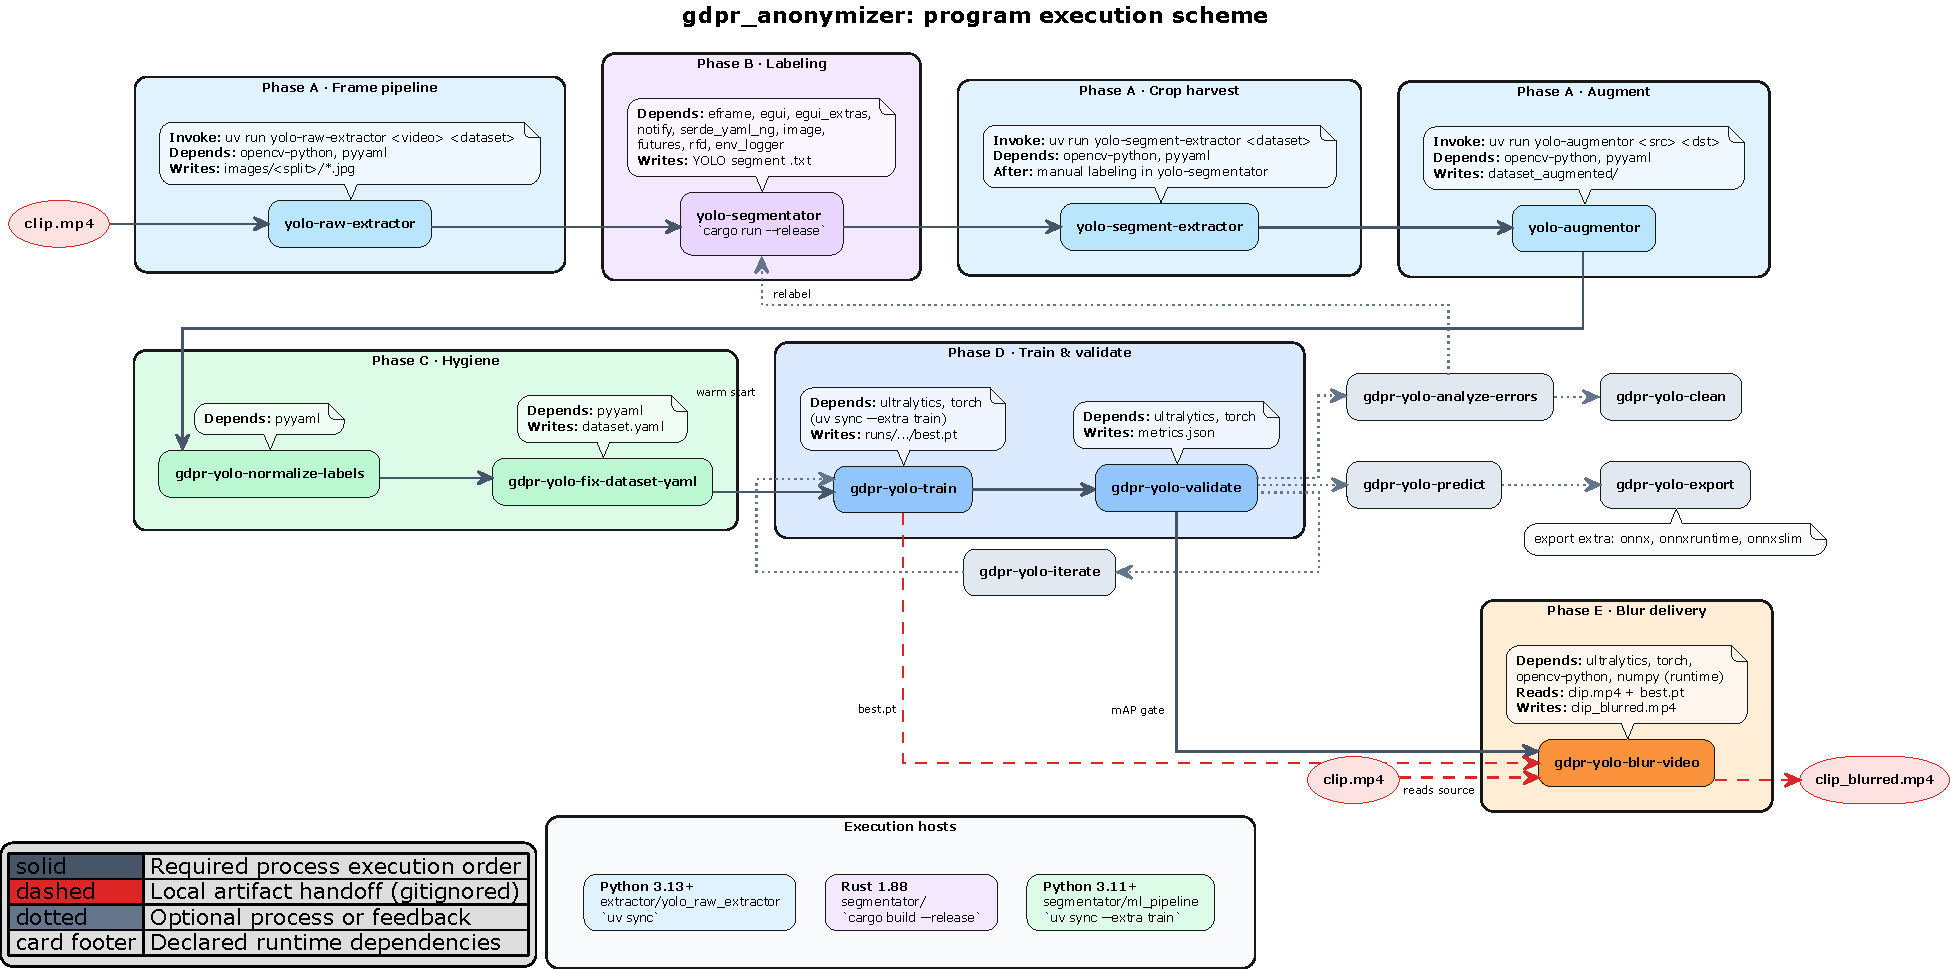
\includegraphics[width=\textwidth]{images/0_program_execution_scheme_manual.pdf}
  \caption{Program execution scheme for \texttt{gdpr\_anonymizer}. Solid arrows denote required process order; dashed arrows denote local artifact handoffs between stages; dotted arrows mark optional or feedback paths. Coloured phase bands group commands by package and runtime host (Python~3.13 extractor, Rust segmentator, Python~3.11 \texttt{ml\_pipeline}).}
  \label{fig:programexecscheme}
\end{figure}

Figure~\ref{fig:programexecscheme} maps the same workflow onto concrete CLI entry points and their runtime dependencies. Command names, flags, and worked examples are documented in the public repository README\footnote{\url{https://github.com/cguerreroto/gdpr_anonymizer/blob/main/README.md}}.
